\begin{document}

\maketitle
\begin{frame}{Outline}
\setcounter{tocdepth}{1}
\tableofcontents
\end{frame}


\section{From Enlightenment to a New world}
\label{sec-1}
\begin{frame}[label=sec-1-1]{Locke and Deists}
\begin{itemize}
\item Nearly all the attitudes of the time came together in John Locke
\item \url{https://www.youtube.com/watch?v=kItXvJLnTtk}
\item Many Deists brought to bear on the biblical miracle stories all the prestige of the scientific discovery of laws
\item Deists distrusted appeals to authority and the miraculous, but they also turned away from anything beyond natural religion in part for moral reasons.
\end{itemize}
\end{frame}
\begin{frame}[label=sec-1-2]{Pietists and Methodists}
\begin{itemize}
\item ``\alert{Enthusiasm}'' was a dirty word in the eighteenth century.
\item story begins in Germany, where Lutheran orthodoxy had increasingly defined faith as assent to a set of doctrines
\item Lutherans suspect any call to moral improvement as a move toward works-righteousness.
\item Methodism with a ``method'' for holiness
\item Wesley and Whitefield changed the shape of popular religion in England and North America, but they made little impact on the attitudes among most intellectuals
\end{itemize}
\end{frame}
\begin{frame}[label=sec-1-3]{The end of Reason}
\begin{itemize}
\item Hume
\item Rousseau
\item Kant
\end{itemize}
\end{frame}
\section{City on a hill}
\label{sec-2}
\begin{frame}[label=sec-2-1]{The city on a hill}
\begin{itemize}
\item the \alert{idea} of \alert{denomination} really developed in the US
\item bewildering variety of developments in US (219)
\end{itemize}
\end{frame}

\begin{frame}[label=sec-2-2]{}
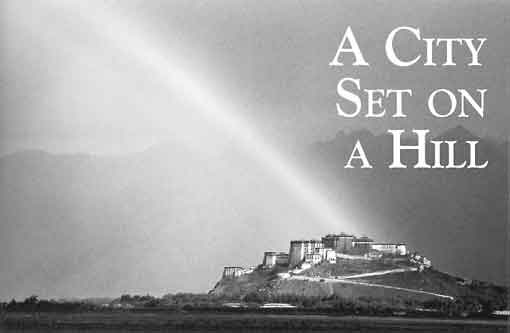
\includegraphics[width=.9\linewidth]{./img/city-on-hill-01.jpg}
\end{frame}

\begin{frame}[label=sec-2-3]{}
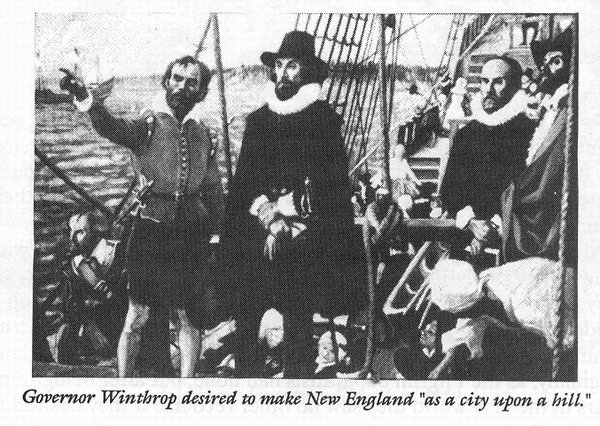
\includegraphics[width=.9\linewidth]{./img/winthrop.jpg}
\end{frame}

\begin{frame}[label=sec-2-4]{}

\includegraphics[width=.9\linewidth]{./img/calvin-resolutions.jpg}
\end{frame}

\begin{frame}[label=sec-2-5]{}
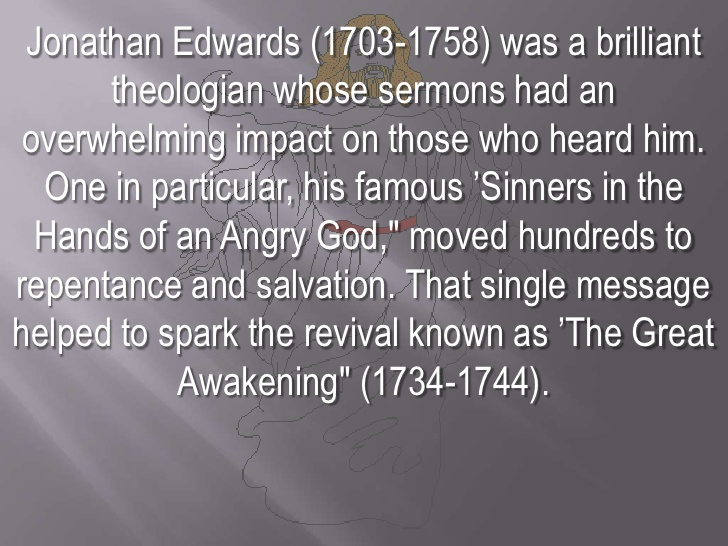
\includegraphics[width=.9\linewidth]{./img/4-prepare-for-action-1-peter-11316-50-728.jpg}
\end{frame}

\begin{frame}[label=sec-2-6]{}

\includegraphics[width=.9\linewidth]{./img/resolution-edwards.jpg}
\end{frame}

\begin{frame}[label=sec-2-7]{}

\includegraphics[width=.9\linewidth]{./img/resolved-to-live.jpg}
\end{frame}

\begin{frame}[label=sec-2-8]{}
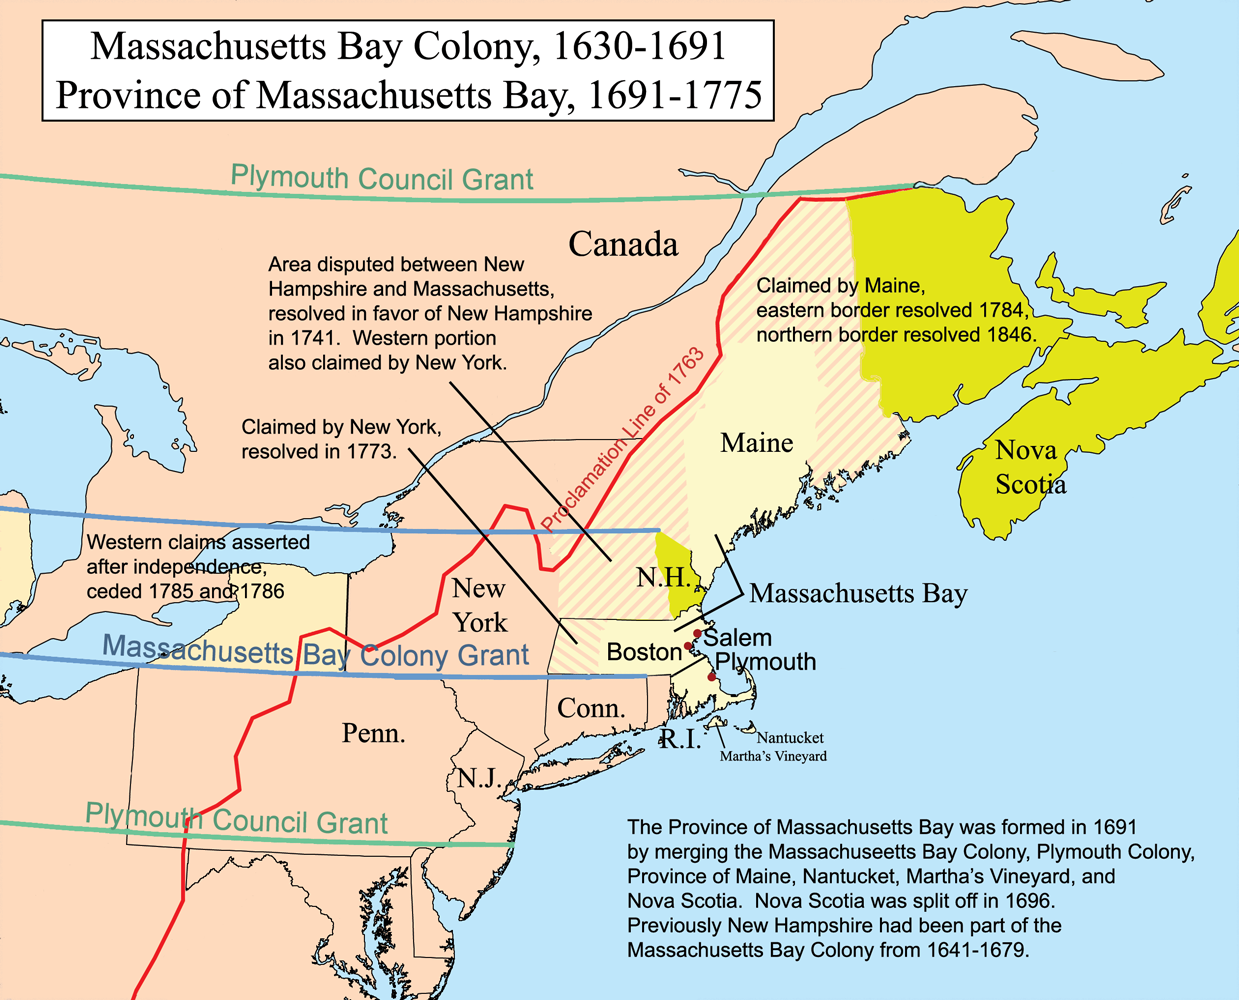
\includegraphics[width=.9\linewidth]{./img/Masscolony.png}
\end{frame}

\begin{frame}[label=sec-2-9]{Key figures}
\begin{itemize}
\item Wesley \& Whitefield
\item John Winthrop
\item Thomas Hooker
\item John Cotton
\item Solomon Stoddard
\item Jonathan Edwards
\begin{itemize}
\item ``Great Awakening''
\end{itemize}
\end{itemize}
\end{frame}

\begin{frame}[label=sec-2-10]{(part 2)}
\begin{block}{Rational Religion}
\begin{itemize}
\item Jefferson \& Franklin
\item William Ellery CHanning
\end{itemize}
\end{block}

\begin{block}{Revivals}
\begin{itemize}
\item Lyman Beecher
\item Charles Finney
\end{itemize}
\end{block}
\begin{block}{Revivals (cont)}
\begin{itemize}
\item Ann Lee \& Quakers
\item Oneida community
\item Latter Day Saints
\item Seventh Day Adventists
\end{itemize}
\end{block}

\begin{block}{Romanticism in America}
\begin{itemize}
\item Unitarians
\begin{itemize}
\item William Ellery Channing
\end{itemize}
\item Transcendentalists
\begin{itemize}
\item Ralph Waldo Emerson
\end{itemize}
\item Nevin \& Schaff (Transform humanity)
\item Horace Bushnell (Attacking individualism)
\end{itemize}
\end{block}

\begin{block}{Slavery \& Black religion}
\begin{itemize}
\item Bushnell
\item Evangelicals in England, Quakers in America
\item the unfulfilled dream of Puritan America
\end{itemize}
\end{block}
\end{frame}
% Emacs 24.3.1 (Org mode 8.2.3c)
\end{document}
